\begin{figure}[t]
    \centering
    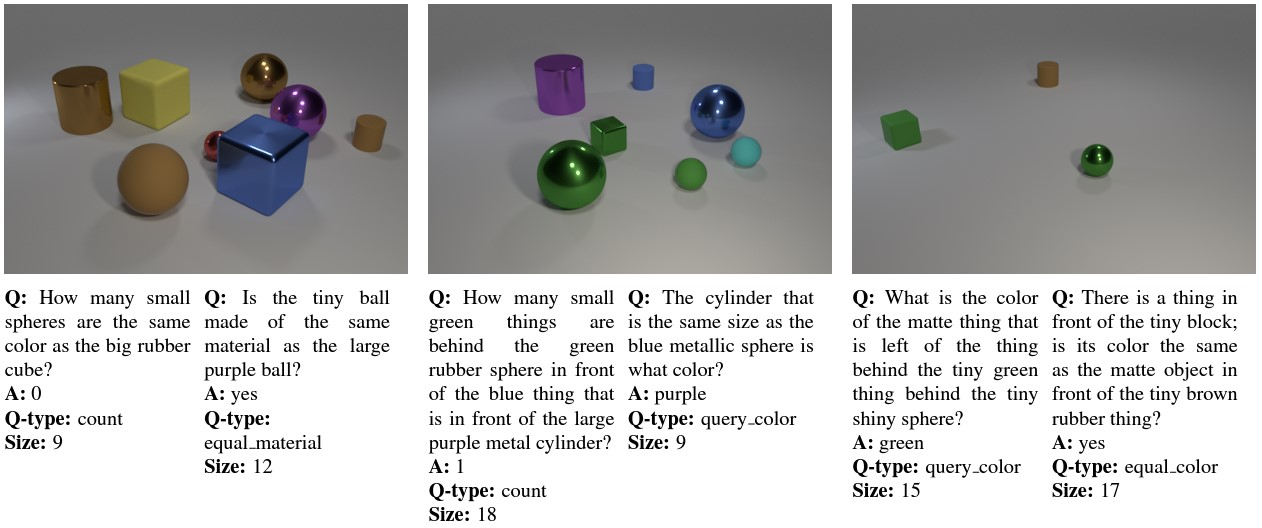
\includegraphics[width=1.0\textwidth]{figures/images/ch2/vqa_problem.jpg}
    \caption{Example of Vision-Question Answering problem get from the CLEVR \cite{johnson2017clevr} dataset. It is possible to observe how for a given image multiple different questions can be done. As well as, questions covers different reasoning skills such as attribute identification, counting, comparison, multiple attention, and logical operations}
    \label{fig:vqa_example}
\end{figure}
